%-*-coding: utf-8-*-

\chapter{Сравнение с другими решениями}
В данной главе будут рассмотрены спроектированные и реализованные решения для поддержки лямбда-функций и функций высших порядков.
Посмотрим как влияют на производительность и память одинаковые конструкции в языках Hack, PHP и KPHP.
Посмотрим какие ошибки стали обнаруживаться при добавление анонимных функций.

\section{Потребление CPU при использовании лямбда-функций}
Давайте рассмотрим время затраченное на различные конструкции.
Начнем с того, сколько времени у нас занимает простое создание лямбда-функций.
Тест представленный в листинге \ref{lst:benchmark-create-simple}, будет в цикле много раз создавать обычную лямбда-функцию, KPHP - не будет оптимизировать простое создание, так как сейчас внутри происходят вызовы функций, находящихся в других единицах трансляции, поэтому тест получится объективными.
\begin{lstlisting}[caption={Бенчмарк создания анонимных функций},label={lst:benchmark-create-simple}]
$n = (int)2e8;
$res = 0;
for ($i = 0; $i < $n; $i++) {
    $f = function($x) { return $x; };
    $res ^= $i;
}
var_dump($res);
\end{lstlisting}

Проделав замер времени работы, получаем следующую картину, показанную на рисунке \ref{fig:benchmark-create-simple}.
Hack представил себя медленнее KPHP всего в 1.3 раза, но эти результаты получились после JIT-а, так например первые 10 запросов к серверу HHVM работали по 12 секунд для теста из листинга \ref{lst:benchmark-create-simple}.
\begin{figure}[H]
    \caption{Сравнение затраченного времени на создание лямбда-функций}
    \label{fig:benchmark-create-simple}
    \centering
    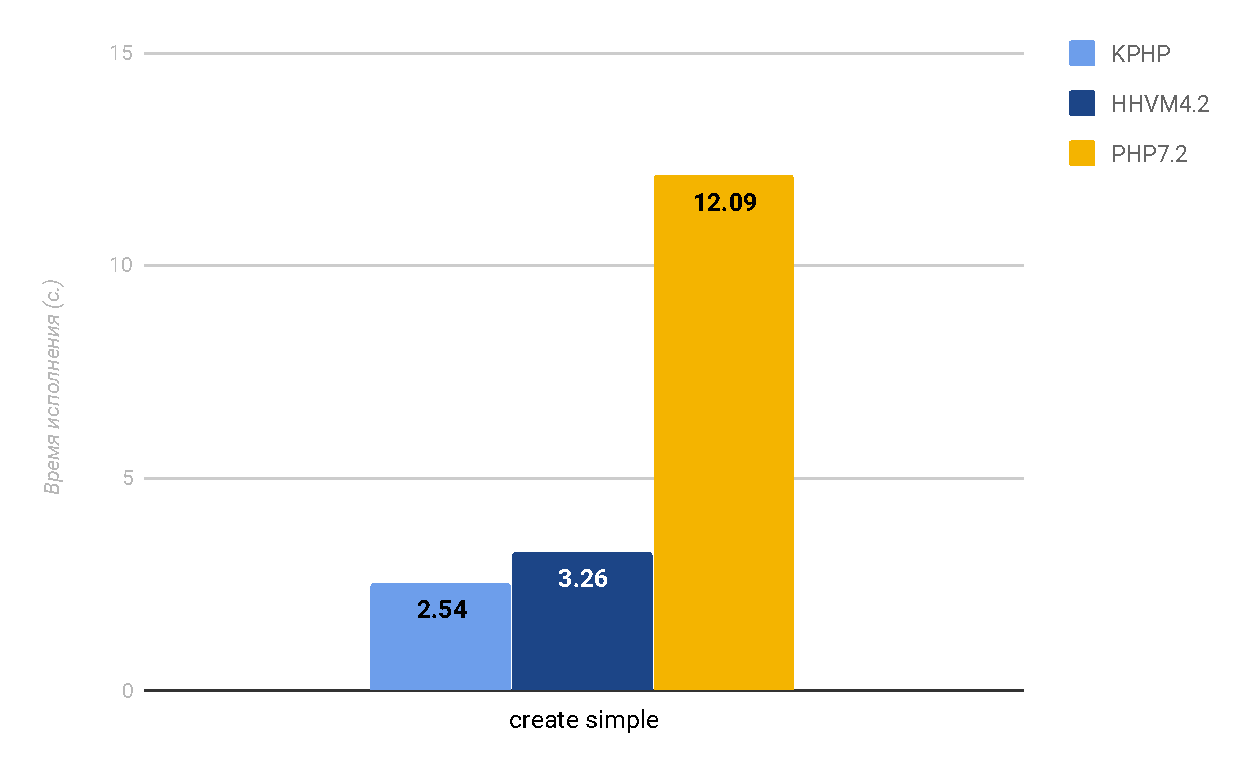
\includegraphics[width=\linewidth]{images/benchmark_create_simple}
\end{figure}

Сравним время которое уходит на вызов созданной лямбда-функции.
Код, который был запущен на всех трех языках представлен в листинге \ref{lst:benchmark-call-simple}.
\begin{lstlisting}[caption={Бенчмарк вызовов анонимных функций},label={lst:benchmark-call-simple}]
$n = (int)2e8;
$res = 0;
$f = function($x) { return $x; };
for ($i = 0; $i < $n; $i++) {
    $res ^= f($i);
}
var_dump($res);
\end{lstlisting}

Результат замеров дал следующие результаты представленные на рисунке \ref{fig:benchmark-call-simple}.
мы видимо как вызов лямбда-функции успешно был встроен в место использования, что привело к нулевым накладным расходам.
\begin{figure}[H]
    \caption{Сравнение затраченного времени на вызов лямбда-функций}
    \label{fig:benchmark-call-simple}
    \centering
    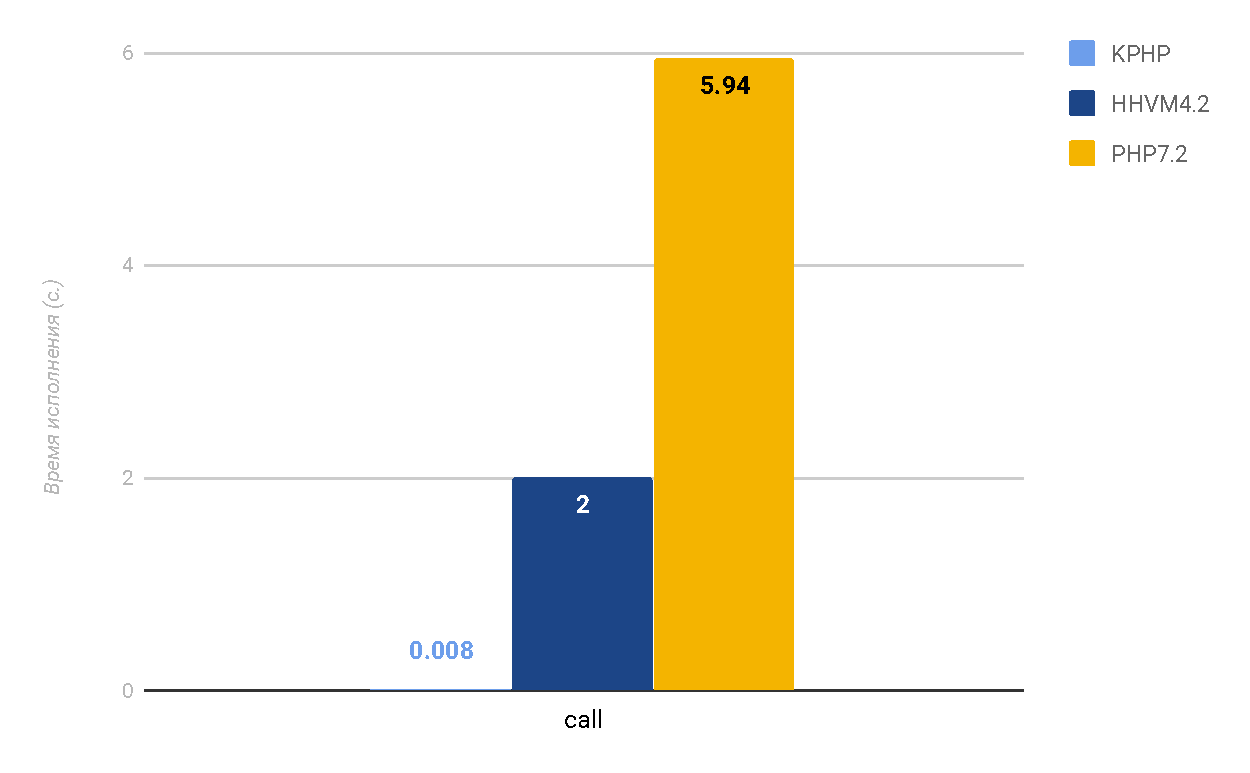
\includegraphics[width=\linewidth]{images/benchmark_call_simple}
\end{figure}

Теперь давайте взглянем на время работы копирования анонимных функций в параметры функций.
Создадим простую лямбда-функцию и будем в цикле ее передавать в другую функцию.
Тест представлен в листинге \ref{lst:benchmark-copy-simple}.
\begin{lstlisting}[caption={Бенчмарк копирования анонимных функций},label={lst:benchmark-copy-simple}]
function foo(callable $f) {}

$n = (int)2e8;
$res = 0;
$f = function($x) { return $x; };
for ($i = 0; $i < $n; $i++) {
    foo($f);
}
var_dump($res);
\end{lstlisting}

На рисунке \ref{fig:benchmark-copy-simple} отчетливо видно, как ссылочная семантика и реализация именно через классы хорошо работает.
У нас получилось дешевым, достаточно скопировать один указатель и увеличить счетчик ссылок, без какой-либо дополнительной мета-информации.
\begin{figure}[H]
    \caption{Сравнение затраченного времени на копирование лямбда-функций}
    \label{fig:benchmark-copy-simple}
    \centering
    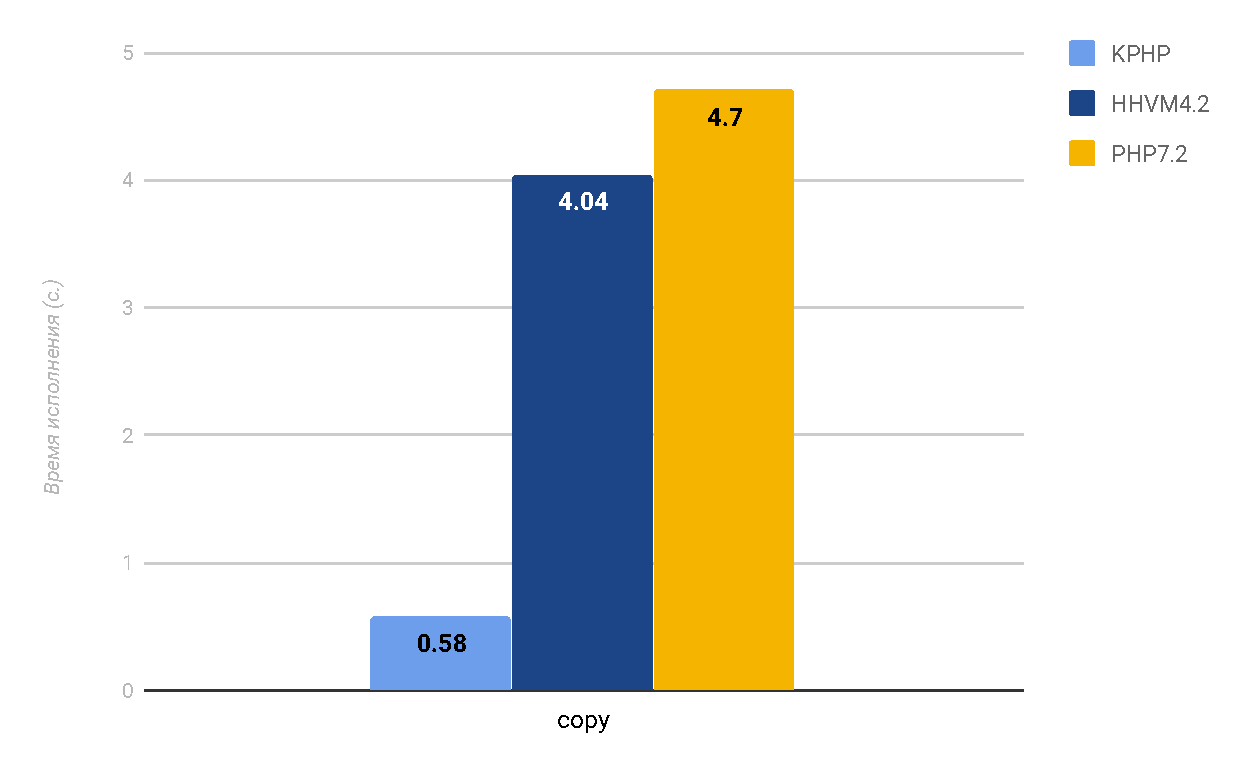
\includegraphics[width=\linewidth]{images/benchmark_copy_simple}
\end{figure}

Также интересно посмотреть на время затраченное при использовании лямбда-функций, которые захватывают переменные из внешнего окружения.
Приведем один общий тест, который сравнивает, сколько времени работает создание и вызов лямбда-функции без захвата переменных и с захватом.
Тест, который запускался на разных языках представлен в листинге \ref{lst:benchmark-create_use_call-simple}, второй запуск был с закомментированной строчкой, которая создают лямбда функции и захватывает переменную.
\begin{lstlisting}[caption={Бенчмарк создания и вызова анонимных функций с захватом},label={lst:benchmark-create_use_call-simple}]
$n = (int)2e8;
$res = 0;
for ($i = 0; $i < $n; $i++) {
    $f = function($x) { return 20 + $x; };
    # $f = function($x) use ($i) { return $i + $x; };
    $res ^= $f($i);
}
var_dump($res);
\end{lstlisting}

На рисунке \ref{fig:benchmark-create_use_call-simple} представлен график сравнения запусков на по очереди заменив использование лямбда-функции с захватом и без.
Диаграмма показывает соотношение времени работы без использования захвата переменных и с использованием.
Можно заметить, что PHP ухудшает производительность почти в 1.5 раза, однако HHVM становится медленнее на 9\%.
В KPHP ничего не меняется, так как компилятор по прежнему справляется встроить лямбда-функцию в место использования и оптимизировать ее.
\begin{figure}[H]
    \caption{Сравнение затраченного времени на создание и вызов анонимных функций с захватом}
    \label{fig:benchmark-create_use_call-simple}
    \centering
    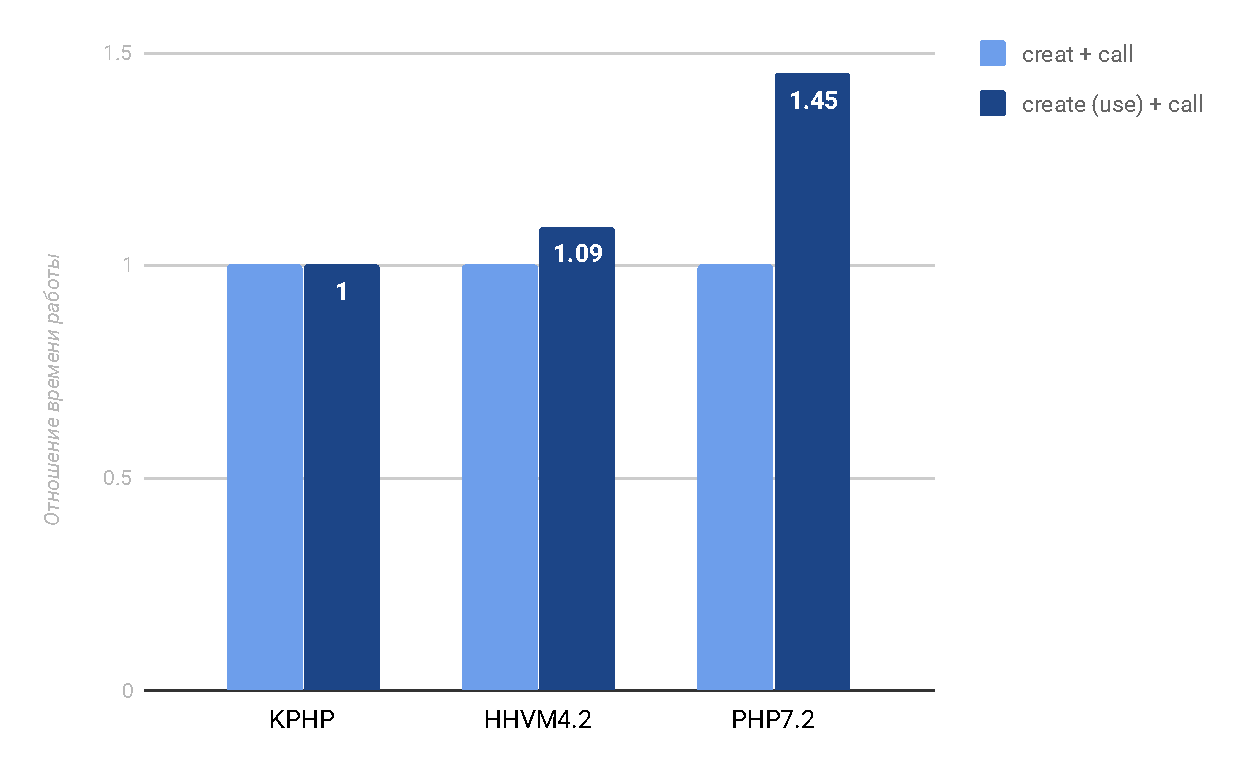
\includegraphics[width=\linewidth]{images/benchmark_create_use_call_simple}
\end{figure}

\section{Потребление CPU при использовании интерфейсов}
Давайте посмотрим на время создания интерфейсов.
Было проведено сравнение, в котором в цикле создавались обычные классы и классы которые реализуют интерфейсы.
Сравнение показало, что в PHP работает в 1.5 раза дольше, а Hack медленнее на целых 18\% процентов.
Также было выявлено, что в PHP и в HHVM создание классов с интерфейсами и без интерфейсов не отличается по времени,
однако в KPHP создание классов с интерфейсами работает на 7-8\% дольше.
Запустив программу вместе с \verb|perf|\cit{perf}, было выявлено, что это происходит из-за виртуальных вызовов функций для подсчета ссылок и освобождения памяти.
Так как в случае интерфейсов эти функции не могут быть девиртуализованны\cite{devirtualization}, то встраивание происходит не так глубоко и оптимизитатор работает хуже, что мы и видим при запуске тестов.

Также было проведено сравнение времени работы вызова виртуальных функций.
С помощью этого механизма будут реализован механизм сохранения разных лямбда-функций в одну переменную.
Результаты оказались такими, что сейчас в KPHP сделано совсем не оптимальным способом работа с интерфейсными методами, так как там при каждом вызове в худшем случае может происходить \verb|n| вызовов \verb|dynamic_cast|, где \verb|n| - это количество классов, реализовавших данный интерфейс.
Данное решение можно достаточно легко соптимизировать, заменив подряд идущие проверки на \verb|switch| по \verb|typeid|\cite{fast-dynamic-cast}, однако сейчас это не требуется.
Тесты показали, что сейчас вызов виртуального метода работает в два раза дольше чем у Hack и всего лишь на 18\% процентов быстрее PHP.
Но в при добавлении возможности сохранять лямбда-функции в одну переменную, конечно же данное решение будет ускорено в разы.


\section{Улучшение качества кода и уменьшение ошибок}
Благодаря тому, что лямбда-функии теперь типизированы, а также типизированы параметры встроенных функций, KPHP начал находить различные ошибки.
Рассмотрим например функцию \verb|usort|.
Она имеет следующую сигнатуру: \verb|usort(&$array, $value_compare_func) : bool| согласно документации PHP.
Принимаемая функция \verb|$value_compare_func| - должна принимать два аргумента и возвращать целое число, меньше нуля, равное нулю, либо большее.

В PHP начиная с 7 версии появилась возможность строгой типизации и подсказывать типы аргументов и возвращаемых значений \cite{php-7-strict-types}.
Так, например, если указать в начале файла \verb|declare(strict_types=1);| то PHP будет во время выполнения выкидывать исключение, если типы не сошлись.
Посмотрим на код в листинге \ref{lst:php-strict-type}.
Там указаны типы принимаемого значения и возвращаемого.
Так как сказана, что функция вернет числовое значение, а она возвращает строку, то во время вызова лямбда-функции PHP выбросит исключение\cite{php-7-pitfalls}.
Конечно таким образом мы можем хотя бы во время исполнения узнать, что типы не сошлись, хотя KPHP еще на этапе компиляции будет ругаться.
\begin{lstlisting}[caption={Пример типизации в PHP7}, label={lst:php-strict-type}]
<?php
declare(strict_types=1);

$f = function (int $x) : int {
  return "Hello";
};

$f(10);
\end{lstlisting}

Вернемся к функции \verb|usort| и взглянем на следующий пример, изображенный в листинге \ref{lst:php-strict-sort}.
\begin{lstlisting}[caption={Пример типизации в PHP7}, label={lst:php-strict-type}]
<?php
declare(strict_types=1);

$a = [0.3, 0.1, 7];

usort($a,
    function(float $x, float $y) : float {
        return $x - $y;
    }
);

var_dump($a);
\end{lstlisting}

Данный пример выведет на экран \verb|[0.3, 0.1, 7]|, то есть сортировка выполнится неверно, а все из-за того, что мы возвращаем из лямбда-функции \verb|float|, хотя по документации требуют возвращать числовое значение.
И конечно разница между \verb|03 - 01| будет равна 0.2, данное значение приведется к числовому значению и превратится в ноль, вместо того, чтобы вернуть число большее нуля, так как 0.3 больше 0.1.

Данный код был также запущен на Hack, именно этот пример отработал у них нормально, хоть по документации и ожидается, что функция должна вернуть целое значение.
Однако заменив разницу на знак меньше и передав лямбда-функцию, которая возвращает \verb|$x < $y|, было получено тоже неверное значение сортировки.
Это показывает, что даже в языке Hack не была поддержана типизация лямбда-функций.
В KPHP все эти примеры не будут компилироваться и мы узнаем о проблеме еще до запуска кода.
Благодаря этому в кодовой базе компании ВКонтакте были найдены десятки ошибок.
Также помимо данной функции есть еще \verb|array_map|, \verb|array_filter| у которых также накладываются ограничения на принимаемые и возвращаемые значения передаваемых лямбда-функций.

\chapterconclusion
Здесь мы сравнили.
Убедились, что наше решение работает в разы лучше аналогов.
Также потребляет меньше памяти.
Находит баги и вообще все супер круто.